% ======================================================================
%  PAC-Former -- CURRENT architecture (AGENT.md sec. 13.43)
%
%  The gauge-invariant MANDATORY PAC interaction tokenizer + tri-axial
%  analytic-signal encoder. This is the configuration that scores
%  TUEV kappa 0.5493 vs the raw-token baseline's 0.4679 (sec. 13.43-I).
%
%  Compile:  pdflatex pac_interaction_architecture.tex   (TikZ, standard libs)
%  (login node has no LaTeX; compile on a compute node or Overleaf.)
%
%  RELATION TO THE OTHER FIGURES IN THIS DIRECTORY
%    mi_architectures.tex        -- v1-v5 PAC-operator mixer line. CLOSED
%                                   (sec. 13.20: pac_scale collapses to 0).
%    triaxial_architecture.tex   -- the raw-token tri-axial backbone. Its
%                                   ENCODER half is still current; its
%                                   FRONTEND (per-(c,b) Conv1d on the filtered
%                                   waveform) is SUPERSEDED by Fig. 1 here.
%
%  WHAT IS NEW, IN ONE SENTENCE
%    Earlier attempts re-weighted an already-complete raw token with PAC and
%    failed (sec. 13.41: mi_product / mi_topk both lost to plain attention).
%    Here PAC DEFINES the token: above the slowest band there is no raw path
%    at all, so the prior cannot be routed around.
%
%  Colour legend:
%    blue   = learnable module (Sinc bank / Conv / Linear / attention / MLP)
%    gray   = parameter-free op (reshape, fold, mean-pool, residual)
%    orange = analytic-signal / physiology path (Hilbert -> phase & amplitude)
%    violet = the measured PAC quantity and the interaction it drives  <-- NOVELTY
%    teal   = positional encoding (electrode xyz, band index)
% ======================================================================
\documentclass[multi=tikzpicture,border=10pt]{standalone}
\usepackage{tikz}
\usepackage{amsmath}
\usetikzlibrary{positioning,arrows.meta,calc,fit,backgrounds,decorations.pathreplacing}

\tikzset{
  box/.style   ={draw, rounded corners=2pt, minimum height=7mm,
                 minimum width=26mm, align=center, font=\footnotesize, thick},
  learn/.style ={box, fill=blue!12,   draw=blue!60},
  op/.style    ={box, fill=black!6,   draw=black!45},
  phys/.style  ={box, fill=orange!18, draw=orange!80},
  pac/.style   ={box, fill=violet!14, draw=violet!70},
  pe/.style    ={box, fill=teal!14,   draw=teal!70},
  io/.style    ={box, fill=black!4,   draw=black!75, minimum width=34mm},
  ctl/.style   ={box, fill=red!6,     draw=red!50, text=red!45!black},
  fl/.style    ={-{Stealth[length=2.4mm]}, thick},
  shp/.style   ={font=\scriptsize\ttfamily, midway, fill=white, inner sep=1pt},
  note/.style  ={font=\scriptsize, align=left},
  eq/.style    ={font=\scriptsize, align=center, fill=violet!5,
                 draw=violet!30, rounded corners=1pt, inner sep=3pt},
  win/.style   ={font=\scriptsize, align=left, fill=green!8,
                 draw=green!45!black, rounded corners=1pt, inner sep=3pt},
}
\newcommand{\nb}{n_b}
\newcommand{\Zij}{Z_{ij}}

\begin{document}

% ======================================================================
% FIGURE 0 -- end-to-end model
% ======================================================================
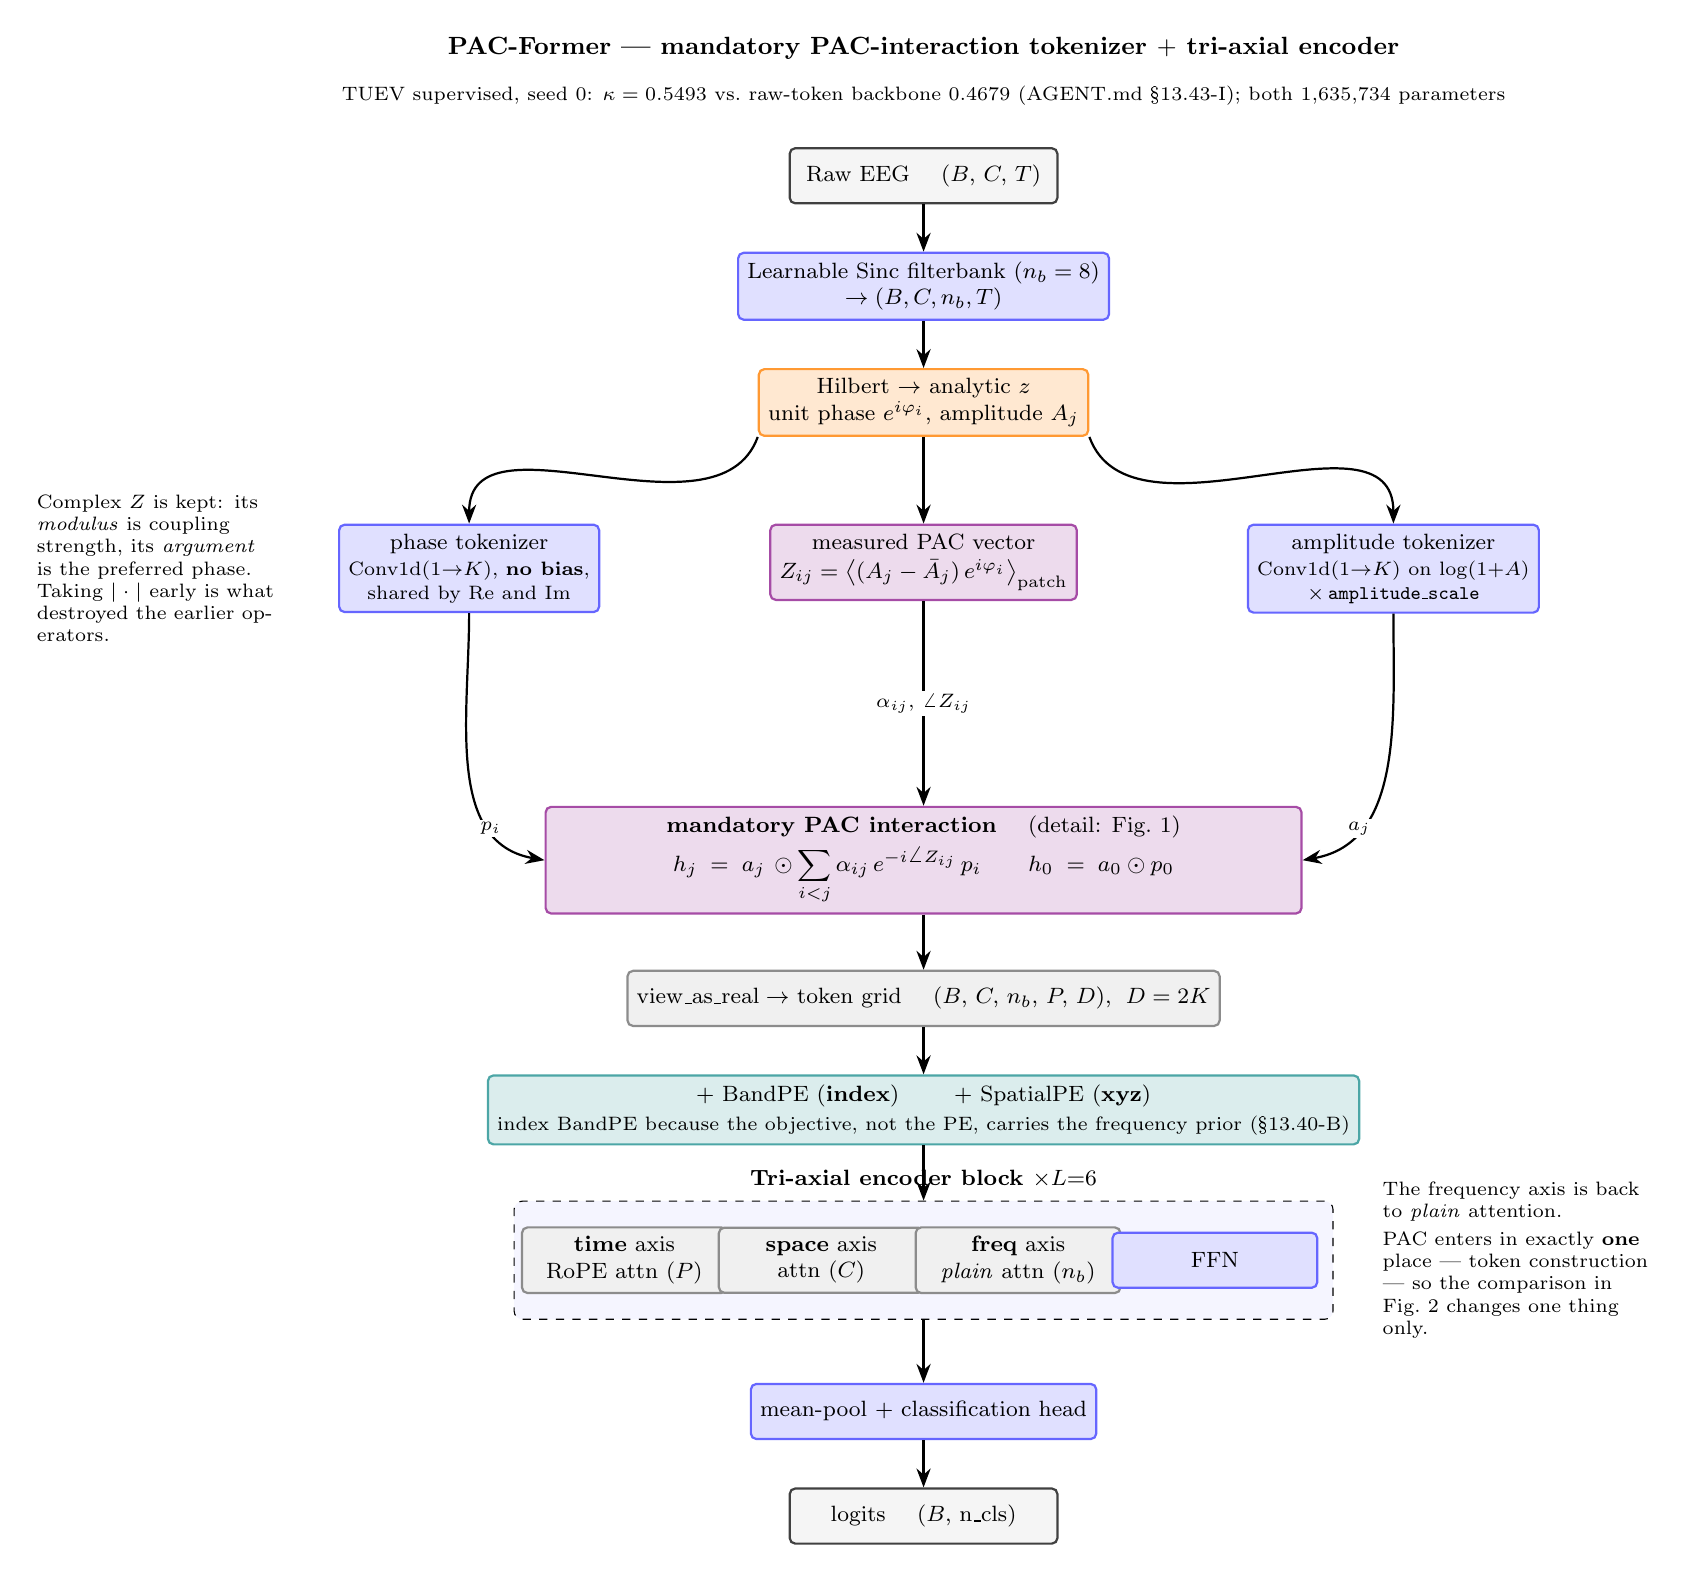
\begin{tikzpicture}[node distance=6mm]
  \node[font=\small\bfseries] (title)
        {PAC-Former --- mandatory PAC-interaction tokenizer $+$ tri-axial encoder};
  \node[font=\scriptsize, below=1mm of title] (sub)
        {TUEV supervised, seed 0: \textbf{$\kappa=0.5493$} vs.\ raw-token backbone $0.4679$
         (AGENT.md \S13.43-I); both $1{,}635{,}734$ parameters};

  \node[io, below=4mm of sub] (raw) {Raw EEG \quad $(B,\,C,\,T)$};

  \node[learn, below=of raw] (sinc)
        {Learnable Sinc filterbank ($\nb=8$)\\ $\to (B,C,\nb,T)$};
  \node[phys, below=of sinc] (hilb)
        {Hilbert $\to$ analytic $z$\\
         unit phase $e^{i\varphi_i}$, amplitude $A_j$};

  % --- the two token paths + the PAC coefficient path ------------------
  \node[learn, below left=11mm and 20mm of hilb] (ptok)
        {phase tokenizer\\ \scriptsize Conv1d$(1{\to}K)$, \textbf{no bias},\\[-1pt]
         \scriptsize shared by $\mathrm{Re}$ and $\mathrm{Im}$};
  \node[learn, below right=11mm and 20mm of hilb] (atok)
        {amplitude tokenizer\\ \scriptsize Conv1d$(1{\to}K)$ on $\log(1{+}A)$\\[-1pt]
         \scriptsize $\times\,\texttt{amplitude\_scale}$};
  \node[pac, below=11mm of hilb] (pacv)
        {measured PAC vector\\[1pt]
         $\Zij=\big\langle (A_j-\bar A_j)\,e^{i\varphi_i}\big\rangle_{\text{patch}}$};

  \node[pac, below=26mm of pacv, minimum width=96mm] (inter)
        {\textbf{mandatory PAC interaction} \quad (detail: Fig.~1)\\[2pt]
         $h_j \;=\; a_j \,\odot \displaystyle\sum_{i<j}\alpha_{ij}\,
          e^{-i\angle \Zij}\,p_i
          \qquad h_0 \;=\; a_0\odot p_0$};

  \node[op, below=7mm of inter] (grid)
        {$\mathrm{view\_as\_real}\to$ token grid \quad $(B,\,C,\,\nb,\,P,\,D)$,\; $D=2K$};

  \node[pe, below=6mm of grid] (pe)
        {$+$ BandPE (\textbf{index}) \qquad $+$ SpatialPE (\textbf{xyz})\\[1pt]
         \scriptsize index BandPE because the objective, not the PE, carries the
         frequency prior (\S13.40-B)};

  \node[draw, dashed, rounded corners=3pt, fill=blue!4,
        minimum width=104mm, minimum height=15mm, below=7mm of pe] (enc) {};
  \node[font=\footnotesize\bfseries, above=0.4mm of enc.north]
        {Tri-axial encoder block $\times L{=}6$};
  \node[op,    at={($(enc.center)+(-38mm,0)$)}] (t)  {\textbf{time} axis\\ RoPE attn ($P$)};
  \node[op,    at={($(enc.center)+(-13mm,0)$)}] (s)  {\textbf{space} axis\\ attn ($C$)};
  \node[op,    at={($(enc.center)+(12mm,0)$)}]  (fq) {\textbf{freq} axis\\ \emph{plain} attn ($\nb$)};
  \node[learn, at={($(enc.center)+(37mm,0)$)}]  (ffn){FFN};

  \node[learn, below=8mm of enc] (head) {mean-pool $+$ classification head};
  \node[io, below=of head] (out) {logits \quad $(B,\,\text{n\_cls})$};

  % --- arrows ---------------------------------------------------------
  \draw[fl](raw)--(sinc);
  \draw[fl](sinc)--(hilb);
  \draw[fl](hilb.south west) to[out=250,in=90] (ptok.north);
  \draw[fl](hilb.south east) to[out=290,in=90] (atok.north);
  \draw[fl](hilb)--(pacv);
  \draw[fl](ptok.south) to[out=270,in=170] node[shp,pos=.75]{$p_i$} (inter.west);
  \draw[fl](atok.south) to[out=270,in=10]  node[shp,pos=.75]{$a_j$} (inter.east);
  \draw[fl](pacv)--node[shp]{$\alpha_{ij},\,\angle \Zij$}(inter);
  \draw[fl](inter)--(grid);
  \draw[fl](grid)--(pe);
  \draw[fl](pe)--(enc);
  \draw[fl](enc)--(head);
  \draw[fl](head)--(out);

  % --- side notes -----------------------------------------------------
  \node[note, right=5mm of enc.east, text width=34mm]
        {The frequency axis is back to \emph{plain} attention.\\[2pt]
         PAC enters in exactly \textbf{one} place --- token construction ---
         so the comparison in Fig.~2 changes one thing only.};
  \node[note, left=5mm of ptok.west, text width=32mm, anchor=east]
        {Complex $Z$ is kept: its \emph{modulus} is coupling strength,
         its \emph{argument} is the preferred phase. Taking
         $|\cdot|$ early is what destroyed the earlier operators.};
\end{tikzpicture}


% ======================================================================
% FIGURE 1 -- the tokenizer, in detail
% ======================================================================
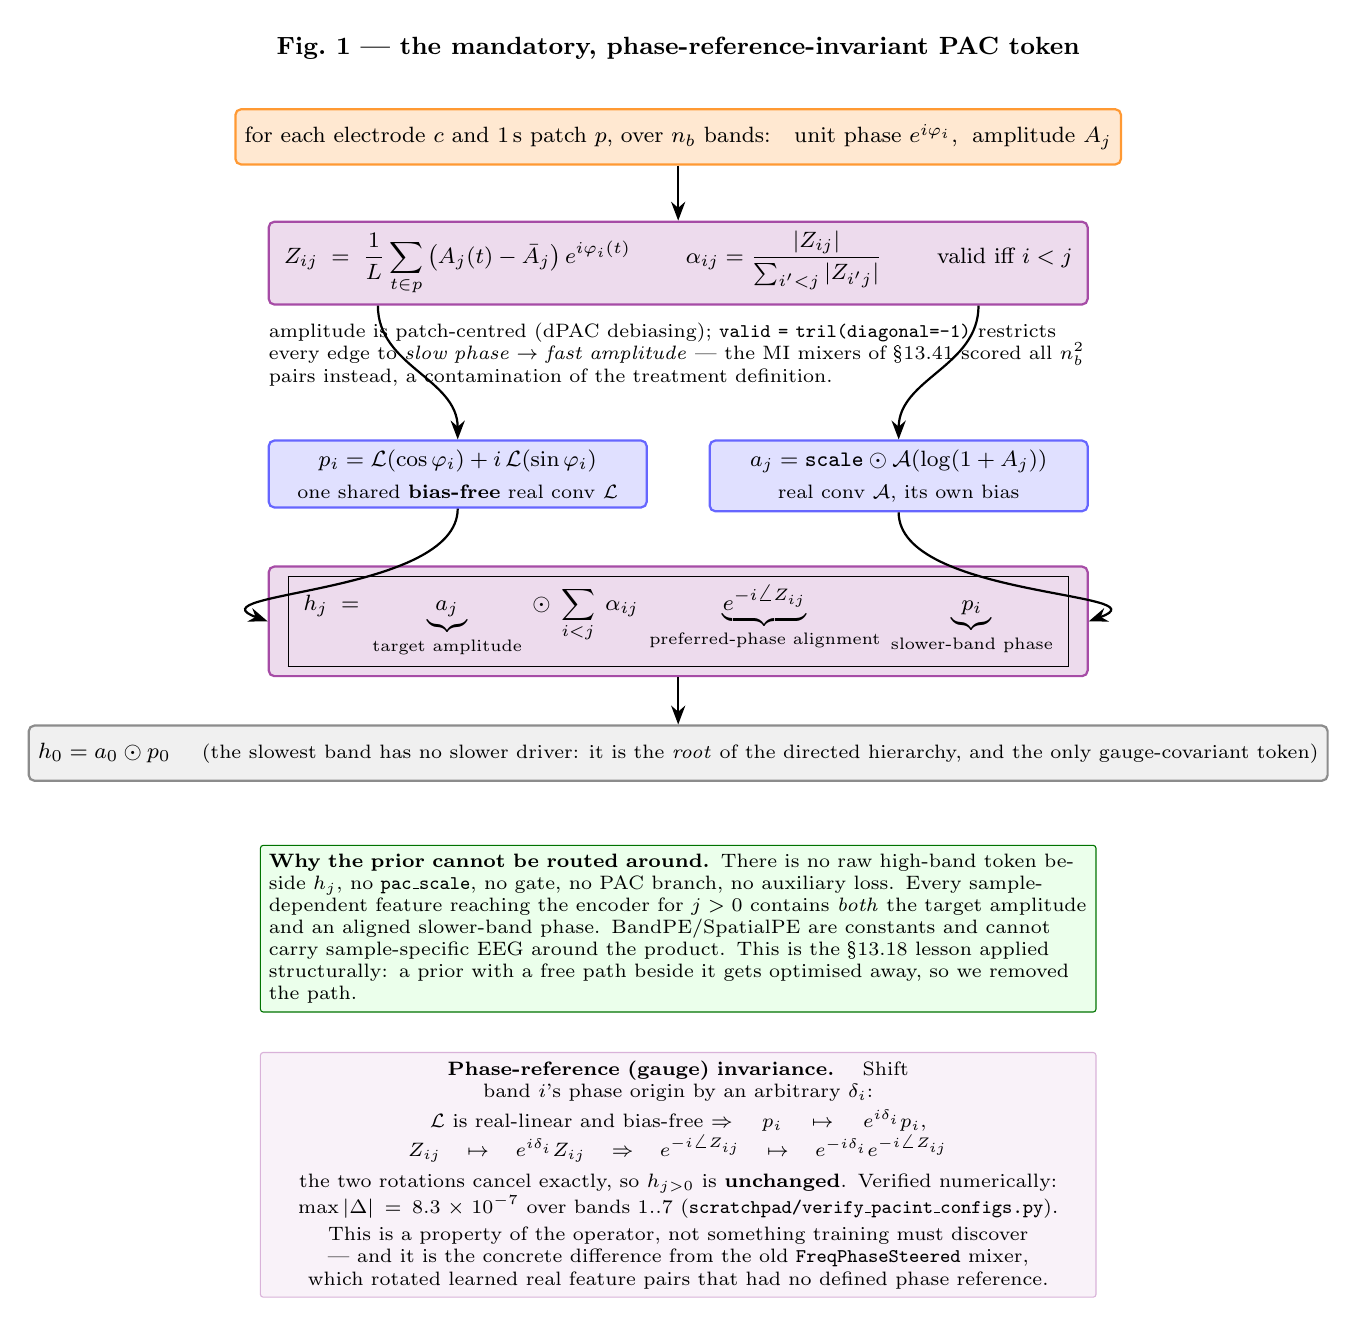
\begin{tikzpicture}[node distance=6mm]
  \node[font=\small\bfseries] (title)
        {Fig.~1 --- the mandatory, phase-reference-invariant PAC token};

  % ---- ingredients ---------------------------------------------------
  \node[phys, below=5mm of title, minimum width=88mm] (ing)
        {for each electrode $c$ and $1\,$s patch $p$, over $\nb$ bands:\quad
         unit phase $e^{i\varphi_i}$,\; amplitude $A_j$};

  \node[pac, below=7mm of ing, minimum width=104mm] (z)
        {$\Zij \;=\; \dfrac{1}{L}\displaystyle\sum_{t\in p}
          \big(A_j(t)-\bar A_j\big)\,e^{i\varphi_i(t)}$
         \qquad
         $\alpha_{ij}=\dfrac{|\Zij|}{\sum_{i'<j}|Z_{i'j}|}$
         \qquad valid iff $i<j$};
  \node[note, below=1mm of z.south, text width=104mm, anchor=north]
        {amplitude is patch-centred (dPAC debiasing); \texttt{valid = tril(diagonal=-1)}
         restricts every edge to \emph{slow phase $\to$ fast amplitude} --- the MI mixers of
         \S13.41 scored all $\nb^2$ pairs instead, a contamination of the treatment definition.};

  % ---- the two features ----------------------------------------------
  \node[learn, below=17mm of z.south west, anchor=north west, minimum width=48mm] (pf)
        {$p_i=\mathcal{L}\!\left(\cos\varphi_i\right)+i\,\mathcal{L}\!\left(\sin\varphi_i\right)$\\[2pt]
         \scriptsize one shared \textbf{bias-free} real conv $\mathcal{L}$};
  \node[learn, below=17mm of z.south east, anchor=north east, minimum width=48mm] (af)
        {$a_j=\texttt{scale}\odot\mathcal{A}\!\left(\log(1+A_j)\right)$\\[2pt]
         \scriptsize real conv $\mathcal{A}$, its own bias};

  % ---- the product ---------------------------------------------------
  \node[pac, below=9mm of z, yshift=-24mm, minimum width=104mm] (h)
        {$\boxed{\;h_j \;=\; \underbrace{a_j}_{\text{target amplitude}}\;\odot\;
          \sum_{i<j}\;\alpha_{ij}\;
          \underbrace{e^{-i\angle \Zij}}_{\text{preferred-phase alignment}}\;
          \underbrace{p_i}_{\text{slower-band phase}}\;}$};
  \node[op, below=6mm of h, minimum width=104mm] (root)
        {$h_0=a_0\odot p_0$ \quad
         \scriptsize (the slowest band has no slower driver: it is the \emph{root} of the
         directed hierarchy, and the only gauge-covariant token)};

  \draw[fl](ing)--(z);
  \draw[fl] ($(z.south west)+(14mm,0)$) to[out=270,in=90] (pf.north);
  \draw[fl] ($(z.south east)+(-14mm,0)$) to[out=270,in=90] (af.north);
  \draw[fl](pf.south) to[out=270,in=160] (h.west);
  \draw[fl](af.south) to[out=270,in=20]  (h.east);
  \draw[fl](h)--(root);

  % ---- why it cannot be bypassed -------------------------------------
  \node[win, below=8mm of root, text width=104mm] (why)
        {\textbf{Why the prior cannot be routed around.}
         There is no raw high-band token beside $h_j$, no \texttt{pac\_scale}, no gate, no
         PAC branch, no auxiliary loss. Every sample-dependent feature reaching the encoder
         for $j>0$ contains \emph{both} the target amplitude and an aligned slower-band phase.
         BandPE/SpatialPE are constants and cannot carry sample-specific EEG around the
         product. This is the §13.18 lesson applied structurally: a prior with a free path
         beside it gets optimised away, so we removed the path.};

  % ---- gauge invariance ----------------------------------------------
  \node[eq, below=5mm of why, text width=104mm] (gauge)
        {\textbf{Phase-reference (gauge) invariance.} \;
         Shift band $i$'s phase origin by an arbitrary $\delta_i$:\\[3pt]
         $\mathcal{L}$ is real-linear and bias-free $\Rightarrow
          p_i\mapsto e^{i\delta_i}p_i$, \qquad
          $\Zij\mapsto e^{i\delta_i}\Zij \Rightarrow
           e^{-i\angle \Zij}\mapsto e^{-i\delta_i}e^{-i\angle \Zij}$\\[3pt]
         the two rotations cancel exactly, so $h_{j>0}$ is \textbf{unchanged}.
         Verified numerically: $\max|\Delta|=8.3\times10^{-7}$ over bands $1..7$
         (\texttt{scratchpad/verify\_pacint\_configs.py}).\\[2pt]
         This is a property of the operator, not something training must discover ---
         and it is the concrete difference from the old \texttt{FreqPhaseSteered} mixer,
         which rotated learned real feature pairs that had no defined phase reference.};
\end{tikzpicture}


% ======================================================================
% FIGURE 2 -- the matched controls and what they isolate
% ======================================================================
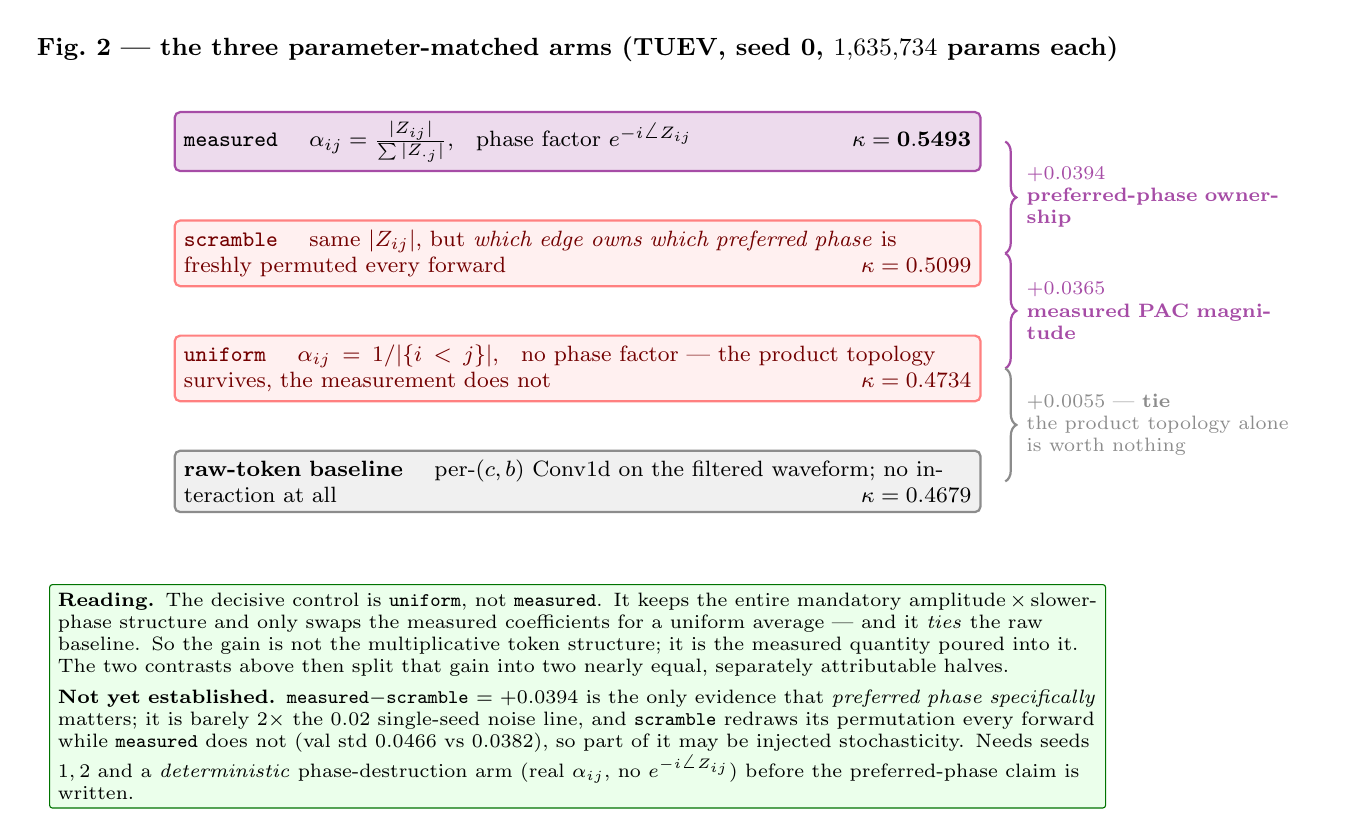
\begin{tikzpicture}[node distance=6mm]
  \node[font=\small\bfseries] (title)
        {Fig.~2 --- the three parameter-matched arms (TUEV, seed 0, $1{,}635{,}734$ params each)};

  % text width (not minimum width) so that \hfill has a box to push against
  \node[pac, below=5mm of title, text width=100mm, align=left] (m)
        {\textbf{\texttt{measured}} \quad
         $\alpha_{ij}=\frac{|\Zij|}{\sum|Z_{\cdot j}|}$, \; phase factor $e^{-i\angle \Zij}$
         \hfill $\kappa=\mathbf{0.5493}$};
  \node[ctl, below=of m, text width=100mm, align=left] (s)
        {\textbf{\texttt{scramble}} \quad
         same $|\Zij|$, but \emph{which edge owns which preferred phase} is freshly permuted
         every forward \hfill $\kappa=0.5099$};
  \node[ctl, below=of s, text width=100mm, align=left] (u)
        {\textbf{\texttt{uniform}} \quad
         $\alpha_{ij}=1/|\{i<j\}|$, \; no phase factor --- the product topology survives,
         the measurement does not \hfill $\kappa=0.4734$};
  \node[op, below=of u, text width=100mm, align=left] (r)
        {\textbf{raw-token baseline} \quad
         per-$(c,b)$ Conv1d on the filtered waveform; no interaction at all
         \hfill $\kappa=0.4679$};

  % brackets showing what each contrast isolates
  \draw[decorate, decoration={brace, amplitude=4pt}, thick, violet!70]
        ($(m.east)+(3mm,0)$) -- ($(s.east)+(3mm,0)$)
        node[midway, right=4pt, note, text width=36mm]
        {$+0.0394$\\ \textbf{preferred-phase ownership}};
  \draw[decorate, decoration={brace, amplitude=4pt}, thick, violet!70]
        ($(s.east)+(3mm,0)$) -- ($(u.east)+(3mm,0)$)
        node[midway, right=4pt, note, text width=36mm]
        {$+0.0365$\\ \textbf{measured PAC magnitude}};
  \draw[decorate, decoration={brace, amplitude=4pt}, thick, black!45]
        ($(u.east)+(3mm,0)$) -- ($(r.east)+(3mm,0)$)
        node[midway, right=4pt, note, text width=36mm]
        {$+0.0055$ --- \textbf{tie}\\ the product topology alone is worth nothing};

  \node[win, below=9mm of r, text width=132mm]
        {\textbf{Reading.} The decisive control is \texttt{uniform}, not \texttt{measured}.
         It keeps the entire mandatory amplitude\,$\times$\,slower-phase structure and only
         swaps the measured coefficients for a uniform average --- and it \emph{ties} the raw
         baseline. So the gain is not the multiplicative token structure; it is the measured
         quantity poured into it. The two contrasts above then split that gain into two
         nearly equal, separately attributable halves.\\[3pt]
         \textbf{Not yet established.} \texttt{measured}$-$\texttt{scramble} $=+0.0394$ is the
         only evidence that \emph{preferred phase specifically} matters; it is barely
         $2\times$ the $0.02$ single-seed noise line, and \texttt{scramble} redraws its
         permutation every forward while \texttt{measured} does not (val std $0.0466$ vs
         $0.0382$), so part of it may be injected stochasticity. Needs seeds $1,2$ and a
         \emph{deterministic} phase-destruction arm (real $\alpha_{ij}$, no
         $e^{-i\angle \Zij}$) before the preferred-phase claim is written.};
\end{tikzpicture}

\end{document}
